
%% bare_jrnl.tex
%% V1.3
%% 2007/01/11
%% by Michael Shell
%% see http://www.michaelshell.org/
%% for current contact information.
%%
%% This is a skeleton file demonstrating the use of IEEEtran.cls
%% (requires IEEEtran.cls version 1.7 or later) with an IEEE journal paper.
%%
%% Support sites:
%% http://www.michaelshell.org/tex/ieeetran/
%% http://www.ctan.org/tex-archive/macros/latex/contrib/IEEEtran/
%% and
%% http://www.ieee.org/
%%*************************************************************************
%% Legal Notice:
%% This code is offered as-is without any warranty either expressed or
%% implied; without even the implied warranty of MERCHANTABILITY or
%% FITNESS FOR A PARTICULAR PURPOSE! 
%% User assumes all risk.
%% In no event shall IEEE or any contributor to this code be liable for
%% any damages or losses, including, but not limited to, incidental,
%% consequential, or any other damages, resulting from the use or misuse
%% of any information contained here.
%%
%% All comments are the opinions of their respective authors and are not
%% necessarily endorsed by the IEEE.
%%
%% This work is distributed under the LaTeX Project Public License (LPPL)
%% ( http://www.latex-project.org/ ) version 1.3, and may be freely used,
%% distributed and modified. A copy of the LPPL, version 1.3, is included
%% in the base LaTeX documentation of all distributions of LaTeX released
%% 2003/12/01 or later.
%% Retain all contribution notices and credits.
%% ** Modified files should be clearly indicated as such, including  **
%% ** renaming them and changing author support contact information. **
%%
%% File list of work: IEEEtran.cls, IEEEtran_HOWTO.pdf, bare_adv.tex,
%%                    bare_conf.tex, bare_jrnl.tex, bare_jrnl_compsoc.tex
%%*************************************************************************


\documentclass[journal]{IEEEtran}
%
% If IEEEtran.cls has not been installed into the LaTeX system files,
% manually specify the path to it like:
% \documentclass[journal]{../sty/IEEEtran}

\usepackage{url}
\usepackage{pgfplots}  % Used to produce graphs.
\usepackage{pgfplotstable} % Used to make graphs from reading tables.
\usepackage{datatool}  % Used to read CSV and make simple table.
\usepackage{listings}  % Show source code.
\usepackage{algorithm}% http://ctan.org/pkg/algorithms
\usepackage{algpseudocode}% http://ctan.org/pkg/algorithmicx
\usepackage{xstring}
\usepackage{caption}


% *** SOURCE CODE (LISTINGS) SETUP ***
\lstloadlanguages{C++} % Load Perl syntax for listings, for a list of other languages supported see: ftp://ftp.tex.ac.uk/tex-archive/macros/latex/contrib/listings/listings.pdf
\lstset{language=C++, % Use Perl in this example
        frame=single, % Single frame around code
        basicstyle=\small\ttfamily, % Use small true type font
        identifierstyle=, % Nothing special about identifiers                                         
        commentstyle=\usefont{T1}{pcr}{m}{sl}\color{MyDarkGreen}\small, % Comments small dark green courier font
        showstringspaces=false, % Don't put marks in string spaces
        tabsize=4, % 4 spaces per tab
        %
        numbers=left, % Line numbers on left
        firstnumber=1, % Line numbers start with line 1
        stepnumber=5, % Line numbers go in steps of 5
        breaklines=true,
        float=*, % Make listing span both columns.
        lineskip=-1ex % Make the list listings single spaced by undoing 2x spacing
}

\newcommand{\cppcode}[2]{
\begin{figure*}
\lstinputlisting[language=C++,caption=#2,label=#1]{#1.cpp}
\end{figure*}
}

\newcommand{\hppcode}[2]{
\begin{figure*}
\lstinputlisting[language=C++,caption=#2,label=#1]{#1.hpp}
\end{figure*}
}

\newcommand{\bashout}[2]{
\begin{figure*}
\lstinputlisting[language=bash, label=#1,caption=#2]{#1.out}
\end{figure*}
}


\ifCLASSINFOpdf
  % \usepackage[pdftex]{graphicx}
  % declare the path(s) where your graphic files are
  % \graphicspath{{../pdf/}{../jpeg/}}
  % and their extensions so you won't have to specify these with
  % every instance of \includegraphics
  % \DeclareGraphicsExtensions{.pdf,.jpeg,.png}
\else
  % or other class option (dvipsone, dvipdf, if not using dvips). graphicx
  % will default to the driver specified in the system graphics.cfg if no
  % driver is specified.
  % \usepackage[dvips]{graphicx}
  % declare the path(s) where your graphic files are
  % \graphicspath{{../eps/}}
  % and their extensions so you won't have to specify these with
  % every instance of \includegraphics
  % \DeclareGraphicsExtensions{.eps}
\fi





\linespread{1.5}
\begin{document}

\title{Laser Patroll Final Report}


\author{Eric~Krause,~\IEEEmembership{Griddle~Master,~Breakfast~Confectionery~Guild,}
        Josh~Moles,~\IEEEmembership{Waffle~Stomper,~Breakfast~Confectionery~Guild,}
        and~Erik~Rhodes,~\IEEEmembership{Eggtravagent~Chef,~Breakfast~Confectionery~Guild}% <-this % stops a space
\thanks{E. Krause is a master of the arts of pancake capture at the Guild.}% <-this % stops a space
\thanks{J. Moles enjoys the art of waffle design.}% <-this % stops a space
\thanks{E. Rhodes does not understand why eggs are not more common in everyone's daily life.}%
\thanks{Manuscript completed for 10 December 2013.}}


% The paper headers
\markboth{Journal of Doctor Robotnik Baking through Sorting,~Vol.~19,~No.~2,~December~2013}%
{Shell \MakeLowercase{\textit{et al.}}: Bare Demo of IEEEtran.cls for Journals}



\maketitle


\begin{abstract}
%TODO: Abstract needs expanding once paper is completed.
This work discusses a benchmarking of four sort algorithms tested against each other for a Portland State University ECE 588 project. The four sorts tested were C++'s \texttt{std::sort}, Quicksort, Merge sort, and Bitonic sort.
\end{abstract}

\begin{IEEEkeywords}
soting, Bitonic sort, Quicksort, Merge sort, class.
\end{IEEEkeywords}

\IEEEpeerreviewmaketitle



\section{Introduction}
\IEEEPARstart{S}{orting} data is a task in computer science that is highly important because it is a very common operation. This report discusses the work done by Laser Patroll [sic] for a team project at Portland State University for the ECE 588 course taught in Fall 2013. The focus of this project was twofold: 
\begin{itemize}
\item First, to either identify parallel sorting algorithms and implement them, or parallelize existing serial (single-threaded) algorithms. 
\item Second, benchmark each of the selected algorithms against each other.  This involved sorting lists of varying lengths using varying numbers of threads, while measuring the relative performance and behavior of the selected algorithms against a known, highly optimized sort, the C++ \texttt{std::sort}.
\end{itemize}

The four algorithms benchmarked and discussed in this report are the C++ \texttt{std::sort}, Quicksort~\cite{Hoare1961}~\cite{Hoare1962}, Merge sort~\cite{Knuth:1998:ACP:280635}, and Bitonic sort~\cite{Batcher1968}. In this report, we first present an overview of these sorting algorithms in Section~\ref{sec:sorting}, then cover the C++ testing framework designed to check the sorted data and gather results in Section~\ref{sec:testing}, and finally present the results of the four algorithms in Section~\ref{sec:results}.

\section{Sorting Algorithms}
\label{sec:sorting}
This section will discuss the four sorting algorithms run.

\subsection{Basic Sort}
Basic sort was implemented by simply passing the data array to \texttt{std::sort}. In no case was it executed in a parallel fashion.

\subsection{Quick Sort}
%TODO: Integrate pseudocode

Quicksort is a partition-exchange sort that uses pivots to reorder elements. While its worst case is $O(n^2)$, Quicksort tends to perform faster than other sorts in the same performance class. Caches improve the sort time substantially, due to Quicksort's tendency to exhibit spatial locality. It can be sorted in place, allowing for less memory usage during the process. 

\begin{figure*}[f]
  \caption{Quicksort Algorithm from http://www.algolist.net/Algorithms/Sorting/Quicksort}
  \centering
  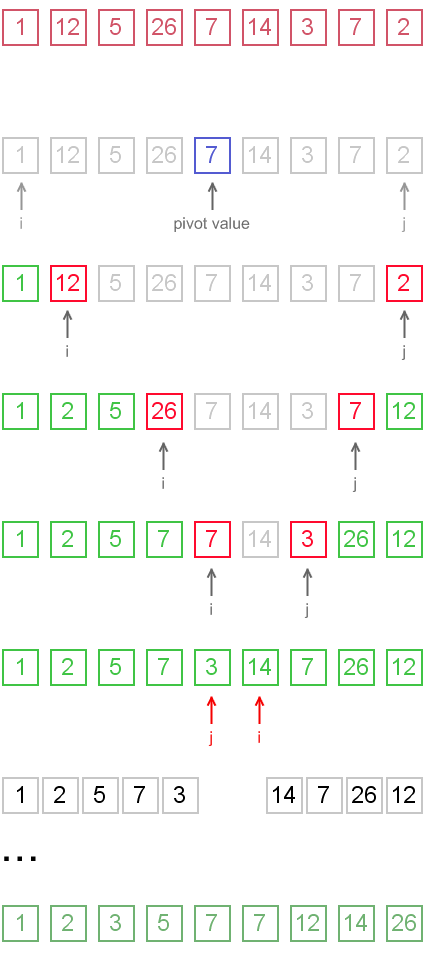
\includegraphics[width=2.5in]{quick-sort.png}
  \label{fig:Quicksort Algorithm}
\end{figure*}

Figure~\ref{fig:Quicksort Algorithm} shows how the sorting is done. First a pivot value is selected.  Starting with the outermost locations, the numbers are compared against the pivot.  After each side has found a number belonging to the other side, the numbers are swapped in place. This is continued until the indexes have switched sides, at which point Quicksort is called recursively.

Quicksort is primarily a sequential algorithm, so to take advantage of parallel threading, the data was divided into different sections by the number of threads available.  This domain decomposition is seen in Figure~\ref{fig:dd}.  Once each thread has finished, they are merged back together and sorted sequentially. 

\begin{figure*}[t]
  \caption{Domain Decomposition}
  \centering
  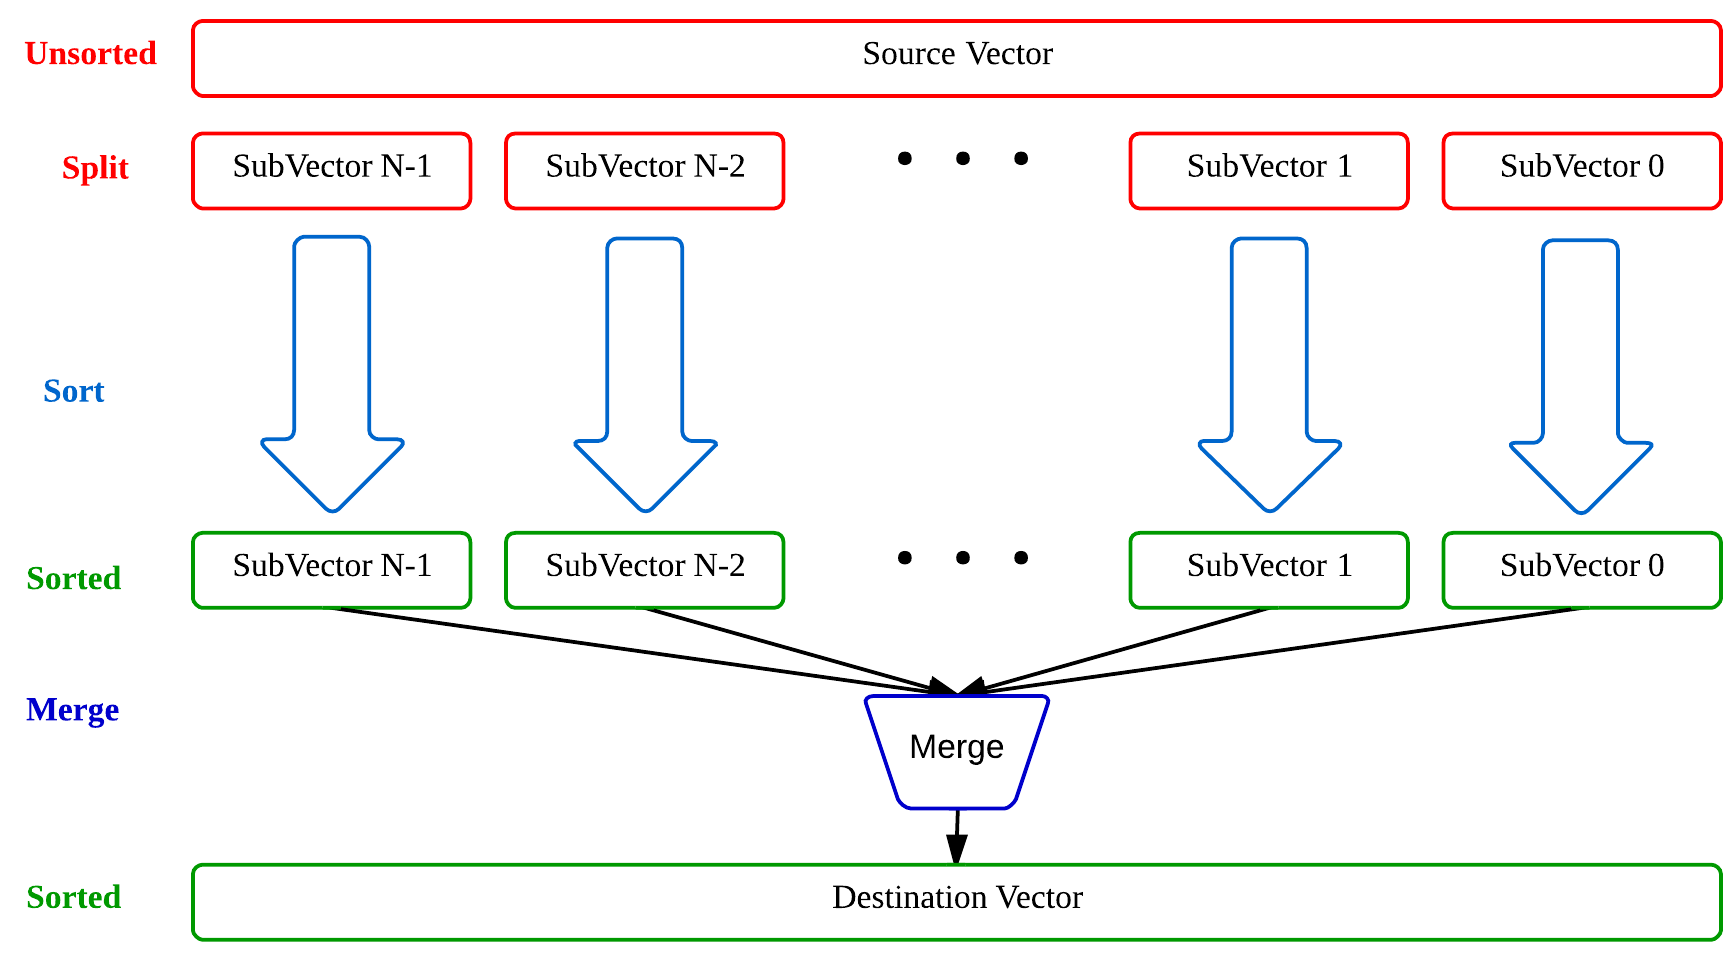
\includegraphics[width=.75\textwidth]{include/dd.png}
  \label{fig:dd}
\end{figure*}


%Parallel Quicksort (data[], num_threads)
%	if (threads > 1)
%		split_data (threads)
%		
%		for (array.length)
%			create_threads
%			
%		for (array.length)
%			join_threads
%			
%		for (threads)
%			merge_threads	
%	else 
%		Quicksort		


% Sequential Quicksort(data[], left, right)
%
%  i = left, j = right
%  while (i <= j) 
%        while (data[i] < pivot)
%              increment i
%        while (data[j] > pivot)
%              decrement j
%        if (i <= j) 
%              swap (data[i], data[j])
%              increment i
%              decrement j
%    
%if (left < j)
%    quickSort(data, left, j)
%if (i < right)
%        quickSort(data, i, right)
%


\subsection{Merge Sort}
Merge sort is a divide-and-conquer sorting algorithm which uniquely exhibits $O(n\ Log(n))$ time complexity regardless of the ordering of its inputs.  The merge algorithm shown in algorithm~\ref{merge} creates a larger sorted array from two smaller sorted subarrays and is pivotal to how merge sort works.  The merge is where the majority of actual work is done when performing a merge sort.   

As shown in algorithm 2, the input array is first split in half until only single elements remain.  Since an array consisting of a single element is inherently sorted, these single elements are then merged together to create increasingly large subarrays, until all subarrays have been merged together in a binary fashion to form a full-sorted result array.

Since splitting the source data is such a fundamental aspect of merge sort, we developed an elegant algorithm which leverages the inherent domain decomposition present in merge sort.  Our method requires no communication between threads, uses no mutexes, and uses a total of only N barriers for N threads.  Furthermore, this algorithm ensures that each thread has access to approximately 1/N of the work and if blocked, is only ever blocked by a single other thread.  

Shown in algorithm~\ref{mms}, Multithreaded Merge Sort (MMS) modifies the merge sort shown in algorithm~\ref{mergesort} to pass in the number of remaining threads.  If this number is zero, MMS functions identically to standard \texttt{mergesort()}. 

If the number of remaining threads is greater than zero however, it means that a new thread will be created to handle one of the two \texttt{mergesort()} calls that MMS will make.  The remaining threads will be decremented by one to reflect the new thread that will be created.  Finally, the number of remaining threads will be divided by two and distributed between the two MMS calls.  Our algorithm always gives the new thread the left half of the input array, and always distributes the remainder of the thread count division to the right.  We measured no change in performance with changes to this convention so it was preserved.  

An example of how MMS would create threads if initially launched with 4 threads is illustrated in Figure~\ref{mms_thread}.  At the top, MMS receives 4 threads. A new thread will be created.  The 3 remaining threads (R) are divided up amongst T\_1, the new thread and the recursive call to MMS performed by T\_0.  As shown, this threading model ensures that every thread has equal access to work at the bottom of the tree once N threads are created.  In this example, each thread is responsible for 2 of the 8 subarrays.  Note that many high-level threads would be blocked for the majority of execution if each call to MMS started (and had to wait on) two threads.

\begin{figure*}[f]
\caption{MMS threading model}
\centering
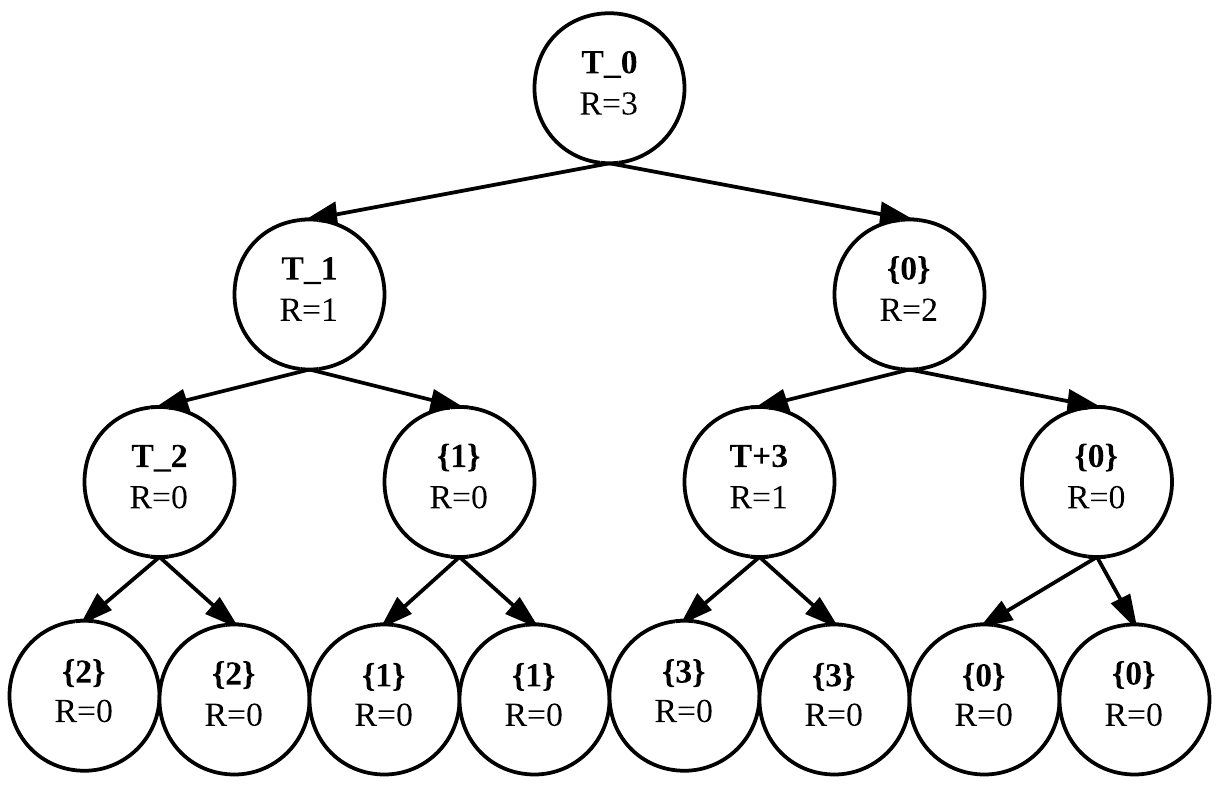
\includegraphics[width=.5\textwidth]{include/mms.png}
\label{mms_thread}
\end{figure*}

\linespread{1}
\begin{algorithm*}[t]
\caption{Merge Algorithm}\label{merge}
\begin{algorithmic}
\Require A,B are sorted arrays
\Require length(dst) = length(A) + length(B)

\Procedure{Merge}{$dst, A, B$}
\State $i, j, k\gets0$ \Comment initialize array indicies
\While{(\emph{i within bounds of A) \textbf{and} (j within bounds of B})} 
	\State $dst[k] \gets \textsc{min}(A[i], B[j]$)
		\State \textit{Increment index of array containing min element (i or j)}	
		\State \textit{Increment k}
\EndWhile
\While{(\emph{i within bounds of A)}} \Comment i still in bounds
	\State $dst[k] \gets A[i]$
	\State \textit{Increment i}
\EndWhile

\While{(\emph{j within bounds of j)}} \Comment j still in bounds
	\State $dst[k] \gets A[j]$
	\State \textit{Increment j}
\EndWhile
\EndProcedure
\end{algorithmic}
\end{algorithm*}

\begin{algorithm*}[t]
\caption{MergeSort Algorithm}\label{mergesort}
\begin{algorithmic}[1]
\Require dst and src are arrays of equal length
\Require low and high are indices into A

\Procedure{MergeSort}{$dst, src, low, high$}

\If {$(low < high)$}
\State \emph {pivot} $\gets$ $\textsc{floor}(low+high)/2$
\State \textsc{MergeSort}$(SortedLeft, A, low, pivot )$\Comment sort left half
\State \textsc{MergeSort}$(SortedRight, A, pivot+1, high)$ \Comment sort right half
\State \textsc{Merge}$(dst,SortedLeft, SortedRight)$\Comment merge left \& right

\EndIf
\EndProcedure
\end{algorithmic}
\end{algorithm*}

\begin{algorithm*}[t]
\caption{Multithreaded Mergesort (MMS)}\label{mms}
\begin{algorithmic}[1]
\Require dst and src are arrays of equal length
\Require low and high are indices into src

\Procedure{MMS}{$dst, src, low, high, threads\_remaining$}


	\If{$threads\_remaining == 0$} \Comment perform basic MergeSort
		\State [perform basic MergeSort algorithm] 
	
	\Else \Comment a new thread will be spawned to sort left
	\If {$(low < high)$}
\State \emph {pivot} $\gets$ $\textsc{floor}(low+high)/2$
	\State \emph{t\_left} = $\textsc{Floor}((threads\_remaining-1)/2)$
	\State \emph{t\_right = t\_left}$ + ((threads\_remaining-1)\%2)$
	\State \emph{New\_Thread}$\gets\emph{\textsc{MMS}(SortedLeft,A,low,pivot, t\_left)}$
	\State \emph{\textsc{MMS}$(SortedRight,A,pivot+1, high, t\_right)$}
	\State \emph{\textsc{Wait}(New\_Thread)}
	\State \emph{\textsc{Merge}$(dst,SortedLeft,SortedRight)$}
\EndIf
\EndIf

\EndProcedure
\end{algorithmic}
\end{algorithm*}
 % put this anywhere that is convenient. it uses exactly 1 page

\subsection{Bitonic Sort}
%TODO: Integrate pseudocode
%Source: wiki.rice.edu.

	\begin{figure*}[t!]
	\caption{Bitonic Split}
  \centering
	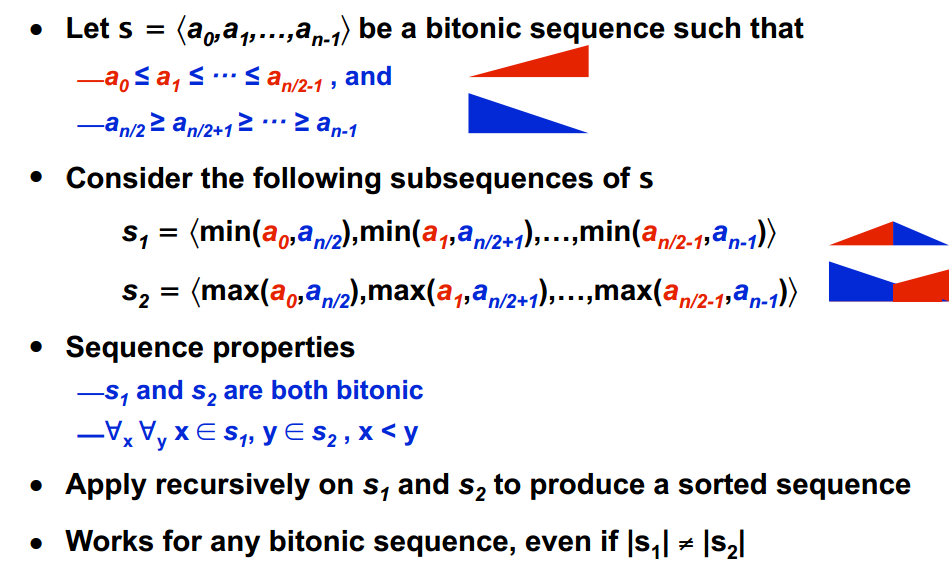
\includegraphics[width=.5\textwidth]{bitonic_split.png}
	\label{bitonic_split}
	\end{figure*}
	
	\begin{figure*}[t!]
	\caption{Bitonic Build}
  \centering
	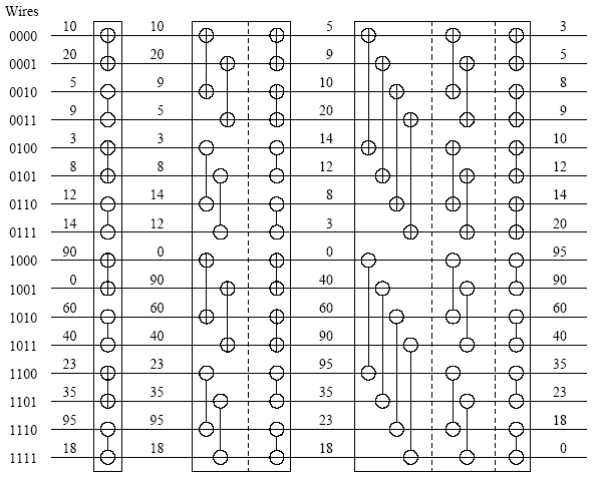
\includegraphics[width=.5\textwidth]{bitonic_build_2.png}
	\label{bitonic_build}
	\end{figure*}

The bitonic sort is a sort algorithm primarily used for parallel execution. The complexity is consistently  $O(n\ Log^2(n))$, regardless of the data received. This sort consists of two different methods.  First, the random data must be sorted or ``built'' into one bitonic sequence.  After this is done, the bitonic sort algorithm is applied and the data is fully sorted (for the sequential version).  

A bitonic sequence consists of sorted data divided into two sections, one with an ascending order and one with a descending order [Figure \ref{bitonic_split}].   Once this has been arranged, the sorting can take place.  To sort the data, each element is compared with the corresponding element of the other half. One half stores the minimum of the compared elements, while the other half stores the maximum number.  Because the bitonic sort uses a divide-and-conquer algorithm, the data is split in half and sorted this way until atomic elements are reached.  

To build the initial bitonic sequence, the bitonic sort is applied to every pair of elements.  It is important to note that if there are only two elements in a dataset, it is guaranteed to be a bitonic sequence.  After this has occurred, each element of the pair is compared with another pair and are sorted down to a single element.  Figure \ref{bitonic_build}~shows how this process is repeated until one large bitonic sequence has been reached.  It is important to note that this sort only works on a data size that is a power of 2.  For this reason, any data of a different was padded to allow the same sorting algorithm to be supplied.
%Mention padding ?

The bitonic sort uses the same algorithm as Quicksort for parallel thread management as shown in Figure~\ref{fig:dd}.

\section{Testing Framework}
\label{sec:testing}

C++ was selected as the language to implement the testing framework and all the sorting algorithms because of the relative ease and ubiquity of tools to compile for the language. The framework had the following objectives for its design:

\begin{itemize}
\item A common path to benchmark each function to ensure timing is measured consistently.
\item Re-usability of common tasks between the sort algorithms.
\item Common call to a Sort function allow blind usage of sort only passing the number of threads and a vector of data.
\item Ability to swap object that data for sorting was stored in easily.
\end{itemize}

\begin{figure*}[t]
  \caption{Framework}
  \centering
  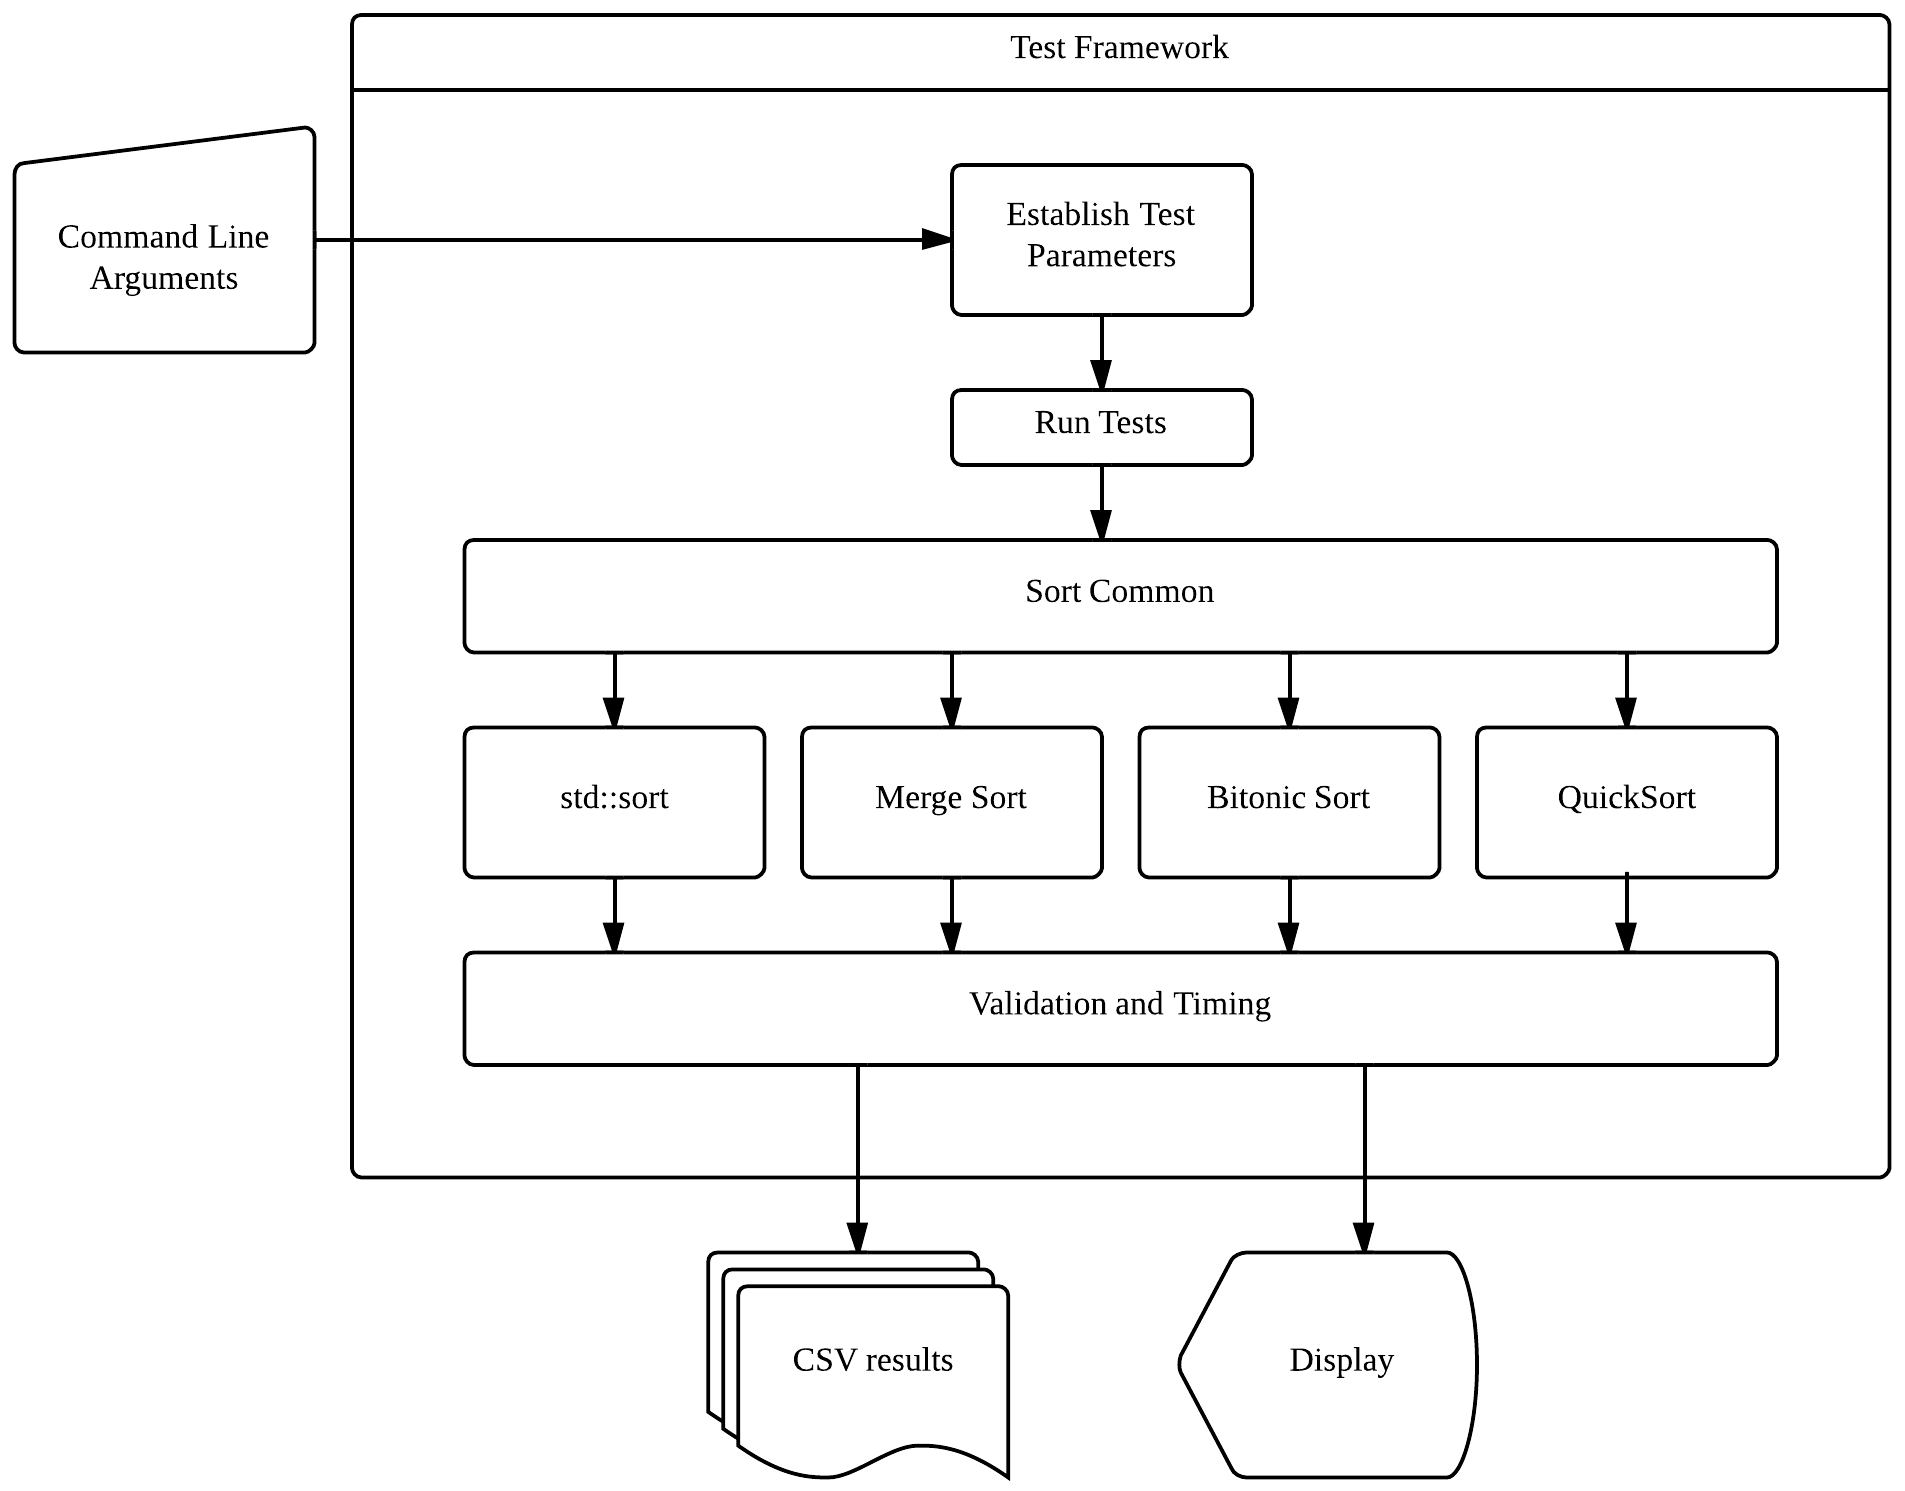
\includegraphics[width=.75\textwidth]{framework.png}
  \label{fig:framework}
\end{figure*}

These goals were accomplished through an object oriented set of classes. A common \texttt{SortCommon} class was the parent of all the sort algorithms and contained the means to benchmark an algorithm, generate an unsorted data vector, check if a given set of data is sorted or not, divide set of data using domain decomposition, merging, and padding (used by Bitonic). Each of the sort functions were free to do the sort by any reasonable means necessary. The requirements were that the only two inputs the Sort gets is a set of data and the number of threads it is allowed to divide the data up across. Figure~\ref{fig:framework} shows the layout of these classes and the overall framework.

The algorithm was to sort the data in place (or at least modify the pointer to the new set of data) so that the benchmark function can then validate that the data was sorted. All four of the algorithms did the sort in place (modified the passed in data directly) or created a ``destination'' data set and then swapped the pointer of the two at the end. Memory utilization can become an issue with sets of data this large so copying or making copies of large subsets of the data was not performed in the algorithms.

C++'s \texttt{std::vector} filled with \texttt{unsigned int} was used as the storage object and data type for each of the algorithms. A \texttt{std::vector} is an efficient, dynamically linked list that was selected over an array for the ability to have an easily growing and shrinking memory space (in case an algorithm selected to do an operation involving such a task). We also feel that the C++ compiler can do a better job optimizing the use of a \texttt{std::vector} in our code compared to the relatively manual task of memory management in an array.

The benchmark function prepared a given set of data to pass to the virtual \texttt{Sort} function implemented by each algorithm. The benchmark function also verified that the data was actually sorted when the \texttt{Sort} function returned. The function only ran the timer for a benchmark of an algorithm during the \texttt{Sort} call portion of the testing. This was done to ensure that any overhead tasks performed by the benchmark function itself does not add to the time a given sort runs.

Data could be generated in a few different patterns depending on the type of sort desired for benchmarking. The three options available were a set of data that is actually in order, a set of data that is in complete reverse, and a set of data that was completely random. The first two were used primarily for verification and testing of aspects of the algorithm. The third (random) set of data was used for all testing shown Section~\ref{sec:results} of the report.

The data was checked for sorting using a single-threaded function to look through the elements. The function simply started at the front of the data and moved through all of the elements. If it found an element that was greater than the previous element (in other words, not sorted), the function would multiply the time it took for the sort to run by $-1$ and print a warning stating that the data was not sorted.

A few other other utility functions were also in the \texttt{SortCommon} class. A function that would take the length of the data and how many threads to divide the work amongst would return a \texttt{std::vector} containing a \texttt{std::pair} of the minimum and maximum index for a given thread to perform the sorting on. Bitonic and Quicksort used this in the functional decomposition of the data, but merge used its own algorithm. For bitonic, the data and the number of threads had to be a power of two without modification. A padding and unpadding function is also added to pad zeros to the data in the event the user requests a sort on data that does not meet the power of two requirement for bitonic.

The code was also checked with valgrind to verify that there were minimal memory leaks. Listing~\ref{valgrind} shows the output from valgrind. The listing shows that the code frees everything of concern (definitely lost).

\bashout{valgrind}{Valgrind Output}

GitHub was also used for revision control. This entire project is available for download at \url{http://github.com/jmoles/laser-patroll/}. Doxygen is also commented in-line to generate a set of HTML and PDF documentation for the project.


\section{Results}
\label{sec:results}
This section provides the results for the tests of the algorithms. The results will show the amount of time it took each algorithm to sort with a varying number of threads and constant data size. It is important to note that throughout all of these tests, anything labeled as ``basic'' is \texttt{std::sort} running in a \textbf{serial} fashion. We did not wrap any parallelization around \texttt{std::sort} so that each of the algorithms are evaluated against the sort that would likely be used in C++.

The results are in Figure~\ref{fig:tvtlg} for a data set of size 134,217,728 elements and Figure~\ref{fig:tvtsm} for a data set of size 512 elements. These tests aimed to see how each algorithm performs with an increasing number of threads both with a small set of data and a large set of data. Ideally, each algorithm should get faster as the number of threads it has available to perform work increases.

Looking first at the large data set, Merge sort follows the ideal situation quite well and starts to reach a limit in execution time as it gets to the end. Quicksort seems fairly flat over the execution regardless of the number of threads allocated to it. This could be a results of the domain decomposition model of splitting up the work and bringing it back together. As the number of threads increases, there is a final merge that only merges two sets of data at a time. This could result in this final merge occupying more time. 

Bitonic is affected by the same merge issue; however, it has another factor slowing it down:  It can only operate on input arrays that are of a length that is a power of 2.  Our Bitonic algorithm pads the inputs data with zeros to increase its length until it is equal to a power of 2, and then removes this additional padding after it is sorted.  Evidently, the amount of time required to pad and unpad the input data is nontrivial, as Bitonic shows an average trend of decreasing execution time, but is susceptible to the requirement that the data and threads must be a power of two. As a result, Bitonic performs the best on the situations where the number of threads is a power of two and begins to slow down as it increases from a power of two, peaking one value right before the next power of two.  

\begin{figure*}[t]
  \centering
  \caption{Time vs Threads Large Data (Size = 134217728)}
  \label{fig:tvtlg}
  \begin{tikzpicture}
    \begin{axis}[
      xlabel={Threads},
      ylabel={Runtime (s)},
      ybar interval,
      width=5.5in,
      filter discard warning=false,
      enlarge y limits=upper,
      enlarge x limits=false,
      legend entries={Basic, Bitonic, Merge, Quick},
      x filter/.code={%
        \ifnum \thisrow{Size} = 134217728
        \else % false
        \def\pgfmathresult{}
        \fi}]
      \addplot table [x=Threads, y=Time, col sep=comma] {data/basic.csv};
      \addplot table [x=Threads, y=Time, col sep=comma] {data/bitonic.csv};
      \addplot table [x=Threads, y=Time, col sep=comma] {data/merge.csv};
      \addplot table [x=Threads, y=Time, col sep=comma] {data/quick.csv};
    \end{axis}
  \end{tikzpicture}
\end{figure*}

\begin{figure*}[t]
  \centering
  \caption{Time vs Threads Large Data (Size = 512)}
  \label{fig:tvtsm}
  \begin{tikzpicture}
    \begin{axis}[
      xlabel={Threads},
      ylabel={Runtime (s)},
      ybar interval,
      width=5.5in,
      bar width=2pt,
      filter discard warning=false,
      enlarge y limits=upper,
      enlarge x limits=false,
      xtick=data,
      legend entries={Basic, Bitonic, Merge, Quick},
      legend pos=north west,
      x filter/.code={%
        \ifnum \thisrow{Size} = 512
        \else % false
        \def\pgfmathresult{}
        \fi}]
      \addplot table [x=Threads, y=Time, col sep=comma] {data/basic.csv};
      \addplot table [x=Threads, y=Time, col sep=comma] {data/bitonic.csv};
      \addplot table [x=Threads, y=Time, col sep=comma] {data/merge.csv};
      \addplot table [x=Threads, y=Time, col sep=comma] {data/quick.csv};
    \end{axis}
  \end{tikzpicture}
\end{figure*}

\section{Conclusion}
The conclusion goes here.


\appendices
% use section* for acknowledgement
\section*{Acknowledgment}


The authors would like to thank...


% Can use something like this to put references on a page
% by themselves when using endfloat and the captionsoff option.
\ifCLASSOPTIONcaptionsoff
  \newpage
\fi

\bibliographystyle{IEEEtran}
% argument is your BibTeX string definitions and bibliography database(s)
%\bibliography{IEEEabrv,../bib/paper}
\bibliography{IEEEabrv,mendeleysources,manualsources}
%
% <OR> manually copy in the resultant .bbl file
% set second argument of \begin to the number of references
% (used to reserve space for the reference number labels box)


% biography section
% 
% If you have an EPS/PDF photo (graphicx package needed) extra braces are
% needed around the contents of the optional argument to biography to prevent
% the LaTeX parser from getting confused when it sees the complicated
% \includegraphics command within an optional argument. (You could create
% your own custom macro containing the \includegraphics command to make things
% simpler here.)
%\begin{biography}[{\includegraphics[width=1in,height=1.25in,clip,keepaspectratio]{mshell}}]{Michael Shell}
% or if you just want to reserve a space for a photo:

\begin{IEEEbiography}{Eric Krause}
%TODO: Type Eric's contribution.
bio
\end{IEEEbiography}

% if you will not have a photo at all:
\begin{IEEEbiography}{Josh Moles}
%TODO: Type Josh's Bio
Biography text here.
\end{IEEEbiography}

% insert where needed to balance the two columns on the last page with
% biographies
%\newpage

\begin{IEEEbiography}{Erik Rhodes}
%TODO: Erik's bio
bio
\end{IEEEbiography}

% You can push biographies down or up by placing
% a \vfill before or after them. The appropriate
% use of \vfill depends on what kind of text is
% on the last page and whether or not the columns
% are being equalized.

%\vfill

% Can be used to pull up biographies so that the bottom of the last one
% is flush with the other column.
%\enlargethispage{-5in}



% that's all folks
\end{document}


